
\iffalse 
Assignment 5
Date    : 6th May 2021
Course  : Applied Programming Lab(EE2703)
Faculty : Prof. Harishankar Ramachandhran

Submission by : Santosh G (EE19B055)

To complie and get the Rep
ort(PDF):
1) python3 EE2703_ASSIGN5_EE19B055.py  (Atleast Once, for the plots)
2) pdflatex EE2703_ASSIGN5_EE19B055.tex
 
PS: Run "EE2703_ASSIGN4_EE19B055.py" using the above command atleast once before running this code, as this program needs the plots.
\fi
\documentclass[11pt, a4paper]{article}
\usepackage{graphicx}
\usepackage{amsmath}
\usepackage[margin=0.6in]{geometry}
\usepackage{listings}
\usepackage{float}

\title{APL(EE2703): Laplace Equation(Assignment 5)} % Title
\author{Santosh G  (EE19B055)} % Author name
\date{\today} % Date for the report

\begin{document}
    \maketitle % Insert the title, author and date

    \section{Aim of the Assignment:}   %Introduction to the assignment
        \begin{itemize}
            \item To find the variation of potential at each point in the given problem statement.
            \item Plot the  potential variation, errors and the current flow
        \end{itemize}
        This shall be achieved by assigning initial values and iterating continuously to reduce the error.
    \section{Introduction}
    The variation in potential can be represented in the following equation:

        \begin{equation}
            \nabla^{2}\phi = \frac{1}{\sigma}\frac{\partial \rho}{\partial t}
        \end{equation}
        \\as we are dealing with DC, the RHS would become Zero. Hence the equation would finally be:
        \\        \begin{equation}
            \nabla^{2}\phi = 0
        \end{equation}        
        \section{Solving}
            \begin{itemize}
    \item
      We are trying to solve for a plate in 2 Dimension hence the above differential equation when considered in 2 dimensions, say x and y, transforms as shown below which can be expanded based of the definitions
          \end{itemize}
    
    \begin{equation}
    \frac{\partial^{2} \phi}{\partial x^{2}}+ \frac{\partial^{2} \phi}{\partial y^{2}} = 0
     \end{equation}
    
    \begin{equation}
    \frac{\partial \phi}{\partial x}_{(x_i,y_j)} = \frac{\phi(x_{i+1/2},y_j) - \phi(x_{i-1/2},y_j)}{\Delta x}
     \end{equation}
    
    \begin{equation}
    \frac{\partial^{2} \phi}{\partial x^{2}}_{(x_i,y_j)} = \frac{\phi(x_{i+1},y_j) -2\phi(x_i,y_j)+ \phi(x_{i-1},y_j)}{(\Delta x)^{2}}
     \end{equation}
    
    \begin{itemize}
    \item
      Using above equations we get
    \end{itemize}
    
    \begin{equation}
            \phi_{i,j} = \frac{\phi_{i+1,j} + \phi_{i-1,j} + \phi_{i,j+1} + \phi_{i,j-1}}{4} 
    \end{equation}
    
    
    \begin{itemize}  % Assumptions and starting conditions
    	\item
      	It is clear that the potential at point can be approximated to the average of potentials at points in the proximity. Hence we start of with values, zero in this condition and keep iterating till the error is less than the tolerance, which happens as the solutions converge. \(Error_k\) denotes the maximum change in elements of \(\phi\) where 'k' is the number of iteration, the error is supposed to be less than some tolerance which is taken as \(10^{-8}\)).

    \item
With the given info of potentials and location of ground we calculateand plot the current flow direction, magnitude etc.
  \end{itemize}
    
	\section{Questions}  % Plots and Hypothesis from the plots
	   \subsection{Contour Plot}
          Plotting the contour plot of the potential.\\
           \\The following is the contour plot of the potentials:
         
            \begin{figure}[H]
                \centering
                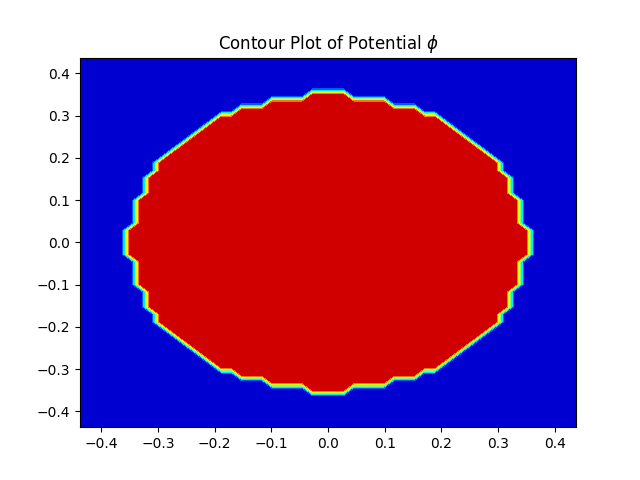
\includegraphics[scale=0.9]{Fig1.png}
                \caption{Contour plot of Potential (Plot for Q1)}                
            \end{figure}
            
	\begin{itemize}
	\item
	 The smoothness increases with increase in \(N_x\) and \(N_y\) as there are more points to smoothen the potential gradient.
       \end{itemize}
	  \subsection{Iterations and Estimations}
	\begin{itemize}
	\item
	 To perform iterations keeping boundary conditions in check
	 \item
	 Boundary Conditions: Due to the abscence of electrodes on three sides the gradient of ptential should be tangential and the normal component should be zero as the cuurent doesnt have any path to flow there after.
	  
       \end{itemize}
        The iterations are performed and the error is calculated. The semilog and loglog plots are plotted as shown below:
         
            \begin{figure}[H]
                    \centering
                    \setlength\tabcolsep{2pt}
                    \begin{tabular}{cc}
                       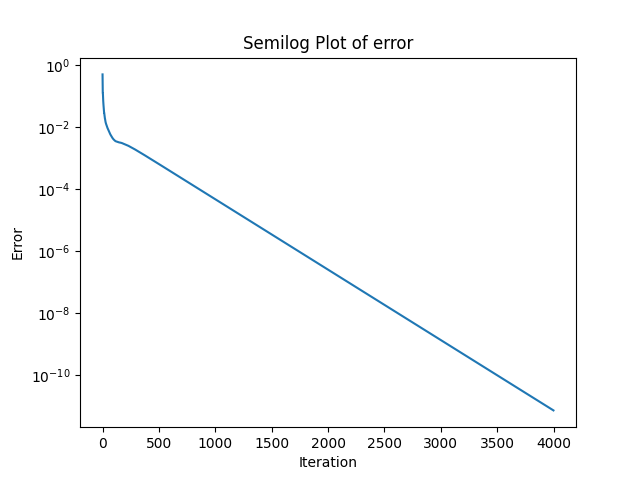
\includegraphics[scale=0.5]{Fig2.png} &
                       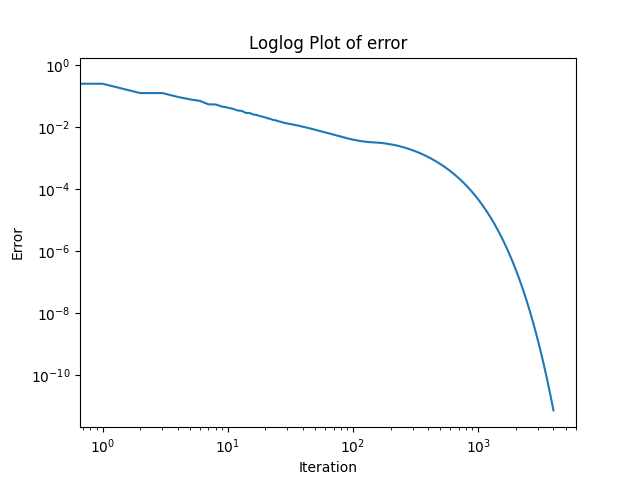
\includegraphics[scale=0.5]{Fig3.png}
                    \end{tabular}
                    \caption{Semilog Plot of Error vs Iterations (Left)} \caption{Loglog plot of Error vs Iterations (Right)}
                \end{figure}
                
          For small number of iterations(1-1000) it is clear from the LogLog plot that log(error) is linearly related to logarith of number of iterations, hence we can conclude the error in this is expoentially varying i.e Error is of the form \(a^x\) where "a" is a constant and "x" corresponds to the number of iterations.\\
          \\ For large number of iterations(2000-6000) the linear relation between the logarithm of error and number of iterations is very clear, hence we can conclude the Error to be of the form \(Ae^{Bx}\), where "A, B" are suitable constants and "x" corresponds to the number of iterations.
            \begin{equation}    
            log(Error) = log(A) + Bx
            \end{equation}
            
            From the above hypothesis, the coefficients are calculated and the deviation(error in estimation) is plotted against number of iterations as shown below.
            
             \begin{figure}[H]
                    \centering
                    \setlength\tabcolsep{2pt}
                    \begin{tabular}{cc}
                       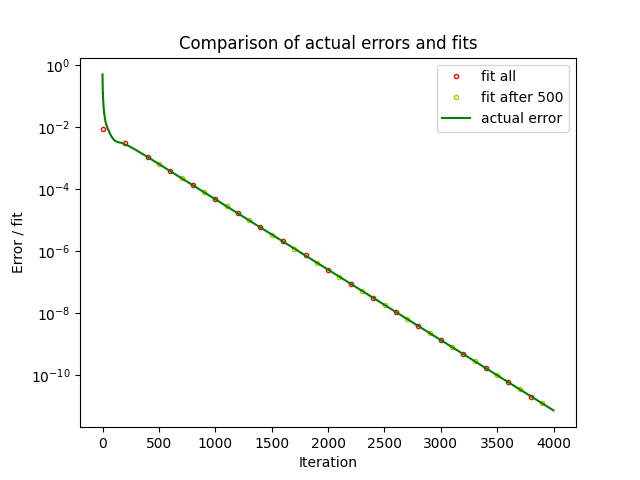
\includegraphics[scale=0.9]{Fig4.png}
                    \end{tabular}
                    \caption{Semilog plot of errors vs Iterations} 
                \end{figure}
 		
 		On solving the following coefficients have been achieved:
 		
		\begin{itemize}
			\item 
			Fit1 : A = 0.00631664 , B = -0.00371103\\
			Fit2 : A = 0.00629419 , B = -0.0037099\\
		\item
		Fit1 is using least squares for all the iterations whereas Fit2 is using lease squares fitting for iterations after the first 500 iterations.
		\item
		It is clear that coefficients in method 1 are larger compared to those in method 2, the deviation between these Fits would increase with number of iterations and it clear Fit2 gives a better approximation at larger number iterations where as both of them would almost be the same at lower number of iterations. This can also be attributed to the fact that we are ignoring the first set of iterations while calculating Fit2.
            
            \end{itemize}

            \subsection{Maximum Error}
           The total error is being calculate dand the magnitudes are summed up as that would result in the maximum error possible, based on this error, the iterations are stopped as there would not be any significant improvement, by still carrying out the iterations.\\
	 \begin{equation}
    		Max Error = \sum_{N+1}^{\infty}error_k
  	\end{equation}

	which can be approximated as follows:

	\begin{equation}
	    Max Error \approx -\frac{A}{B}exp(B(N+0.5))
    	\end{equation}
    	
    	N corresponds to the iteration Number.
    	
    	\begin{itemize}                
          \item
          On calculating, N = 3179 is the result obtained when the total is error is around \(9.98 \times 10^{-8}\) 
          \item
          The last observed change after iteration is \(5.25 \times 10^{-10}\)
          \item
          Though the change per iteration is small, the iterations are continuous summing to a significantly larger error adn would also increase the time, hence being known as one of the worst possible ways to slove it.
        \end{itemize}  
           
        \subsection{Surface plot and Contour plot of potential}
        
        We need to plot the surface potential and the contour plot of the potentials, Based on the diagrams, necessary hypothesis is to be made.\\
        \\The diagrams are plotted as shown below:   
                 \begin{figure}[H]
                    \centering
                    \setlength\tabcolsep{2pt}
                    \begin{tabular}{cc}
                       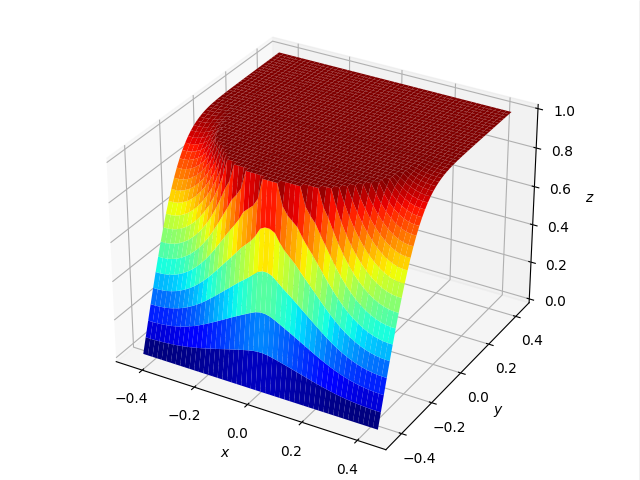
\includegraphics[scale=0.9]{Fig5.png}
                    \end{tabular}
                    \caption{3-D surface  plot of potential} 
                \end{figure}
 		
 		\begin{figure}[H]
                    \centering
                    \setlength\tabcolsep{2pt}
                    \begin{tabular}{cc}
                       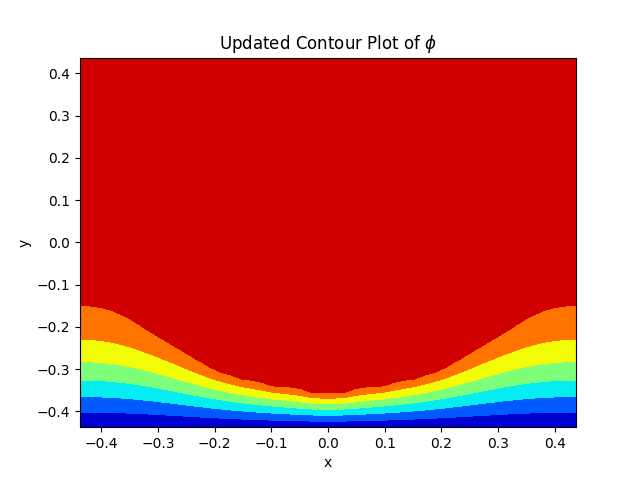
\includegraphics[scale=0.9]{Fig6.png}
                    \end{tabular}
                    \caption{Contour plot of potential} 
                \end{figure}
 		
           \begin{itemize}
           \item
           From Figure 6 it is very clear that there is very little potential on the top and sides of the plate as there is no electrode attached and hence current has no path to flow. As the current cannot flow, the potential wouldn't change and almost remaons constant.
           \item
           The bottom side of the plate is attached to the ground and clearly provides a path for the current to flow hence there is clear drop in potential.
           \item
           As most of the current flows through the bottom part of the plate and flowing of current causes heating, the bottom part would heat up the most and hence would be at the highest temperature throughout the plate.
           
           \end{itemize}
           
     \subsection{Vector plot of Currents}
        
       Based on the potential and their gradienst calculated we can measure the current, both in terms of magnitude and direction, those pbtained results are being plotted in the diagrams below:   
                 \begin{figure}[H]
                    \centering
                    \setlength\tabcolsep{2pt}
                    \begin{tabular}{cc}
                       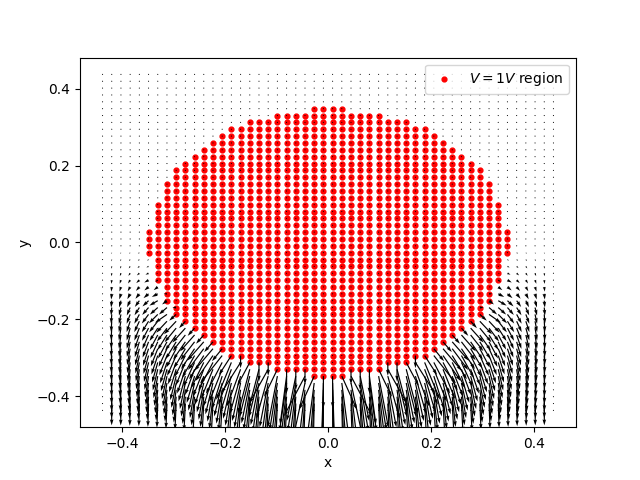
\includegraphics[scale=0.9]{Fig7.png}
                    \end{tabular}
                    \caption{Vector Plot of currents} 
                \end{figure}
 	
 	The red dots corresponds to places where the potential is 1V, i.e corresponds to the source wire and points of plate in close proximity to the wire. 
 		
           \begin{itemize}
           \item
           As discussed previously. most of the current flows through the bottom side of the plate and hence we can see large current density flowing through the bottom side and very little(almost zero) current density on the othe other sides.          
           \end{itemize}
                      
    \section{Conclusion}
    \begin{itemize}
    \item
    Increasing number of iteration while calculations increases the accuracy of the fit by reducing the error, increasing the points considered(\(N_x\) and \(N_y\)) would also improve the effiency.
    
    \item
    By increasing the number of iterations would increase the time for calculations, hence there is a trade-off between the time taken and accuracy of the fit
    
    \item
    Most of the current passes through bottom side of the plate as there is complete path for current to flow unlike the other sides of the plate.
    \item
    The current flow causes heating of the bottom side and hence resulting in higher temperature on the bottom side of the 
    
    \end{itemize}    
\end{document}
